\documentclass[main.tex]{subfiles}

\begin{document}

\section{Testing and Verification}

\textit{This chapter will go over the simulations created for the purpose of testing IPbus and control software, as well as tests performed for the Power Control System prototype. Testing methods and test coverage will be analyzed and discussed and also methods for error prevention will be discussed. Test scripts have been created to test and verify the various parts of the \gls{pcs} and control software and the results will be discussed in this chapter.}

Testing and verification is one of the most important and potentially time consuming parts of the design process. It is essential while in the design process to create not only tests for your system, but also ensure the system is easy to test. This chapter will go over the different tests performed on control software, \gls{fpga} and microcontroller of the \gls{mb}.

\subsection{Test setup}
\label{ssec: test_setup}

The development of the \gls{dtc} is still undergoing and as such, we do not have access to the \gls{alpide} layers, nor do we have the necessary hardware to set up all 43 monitor boards for the \gls{pcs}. The design of the \gls{mb} is still not complete and setting up the full \gls{pcs} is therefore still not viable.

We can however set up a prototype of the \gls{pcs} that will be in practice, identical to the final product, but without connection to the actual sensors. This prototype is realized with a computer connected to the KCU105 evaluation board, and pins on the board is connected to the \gls{usart} signals. The \gls{usart} signals is then wired to a microcontroller development kit, programmed with the \gls{mb} software. An image of the prototype is shown in \autoref{fig: pcs_setup}.

\begin{figure}[!htpb]
    \centering
    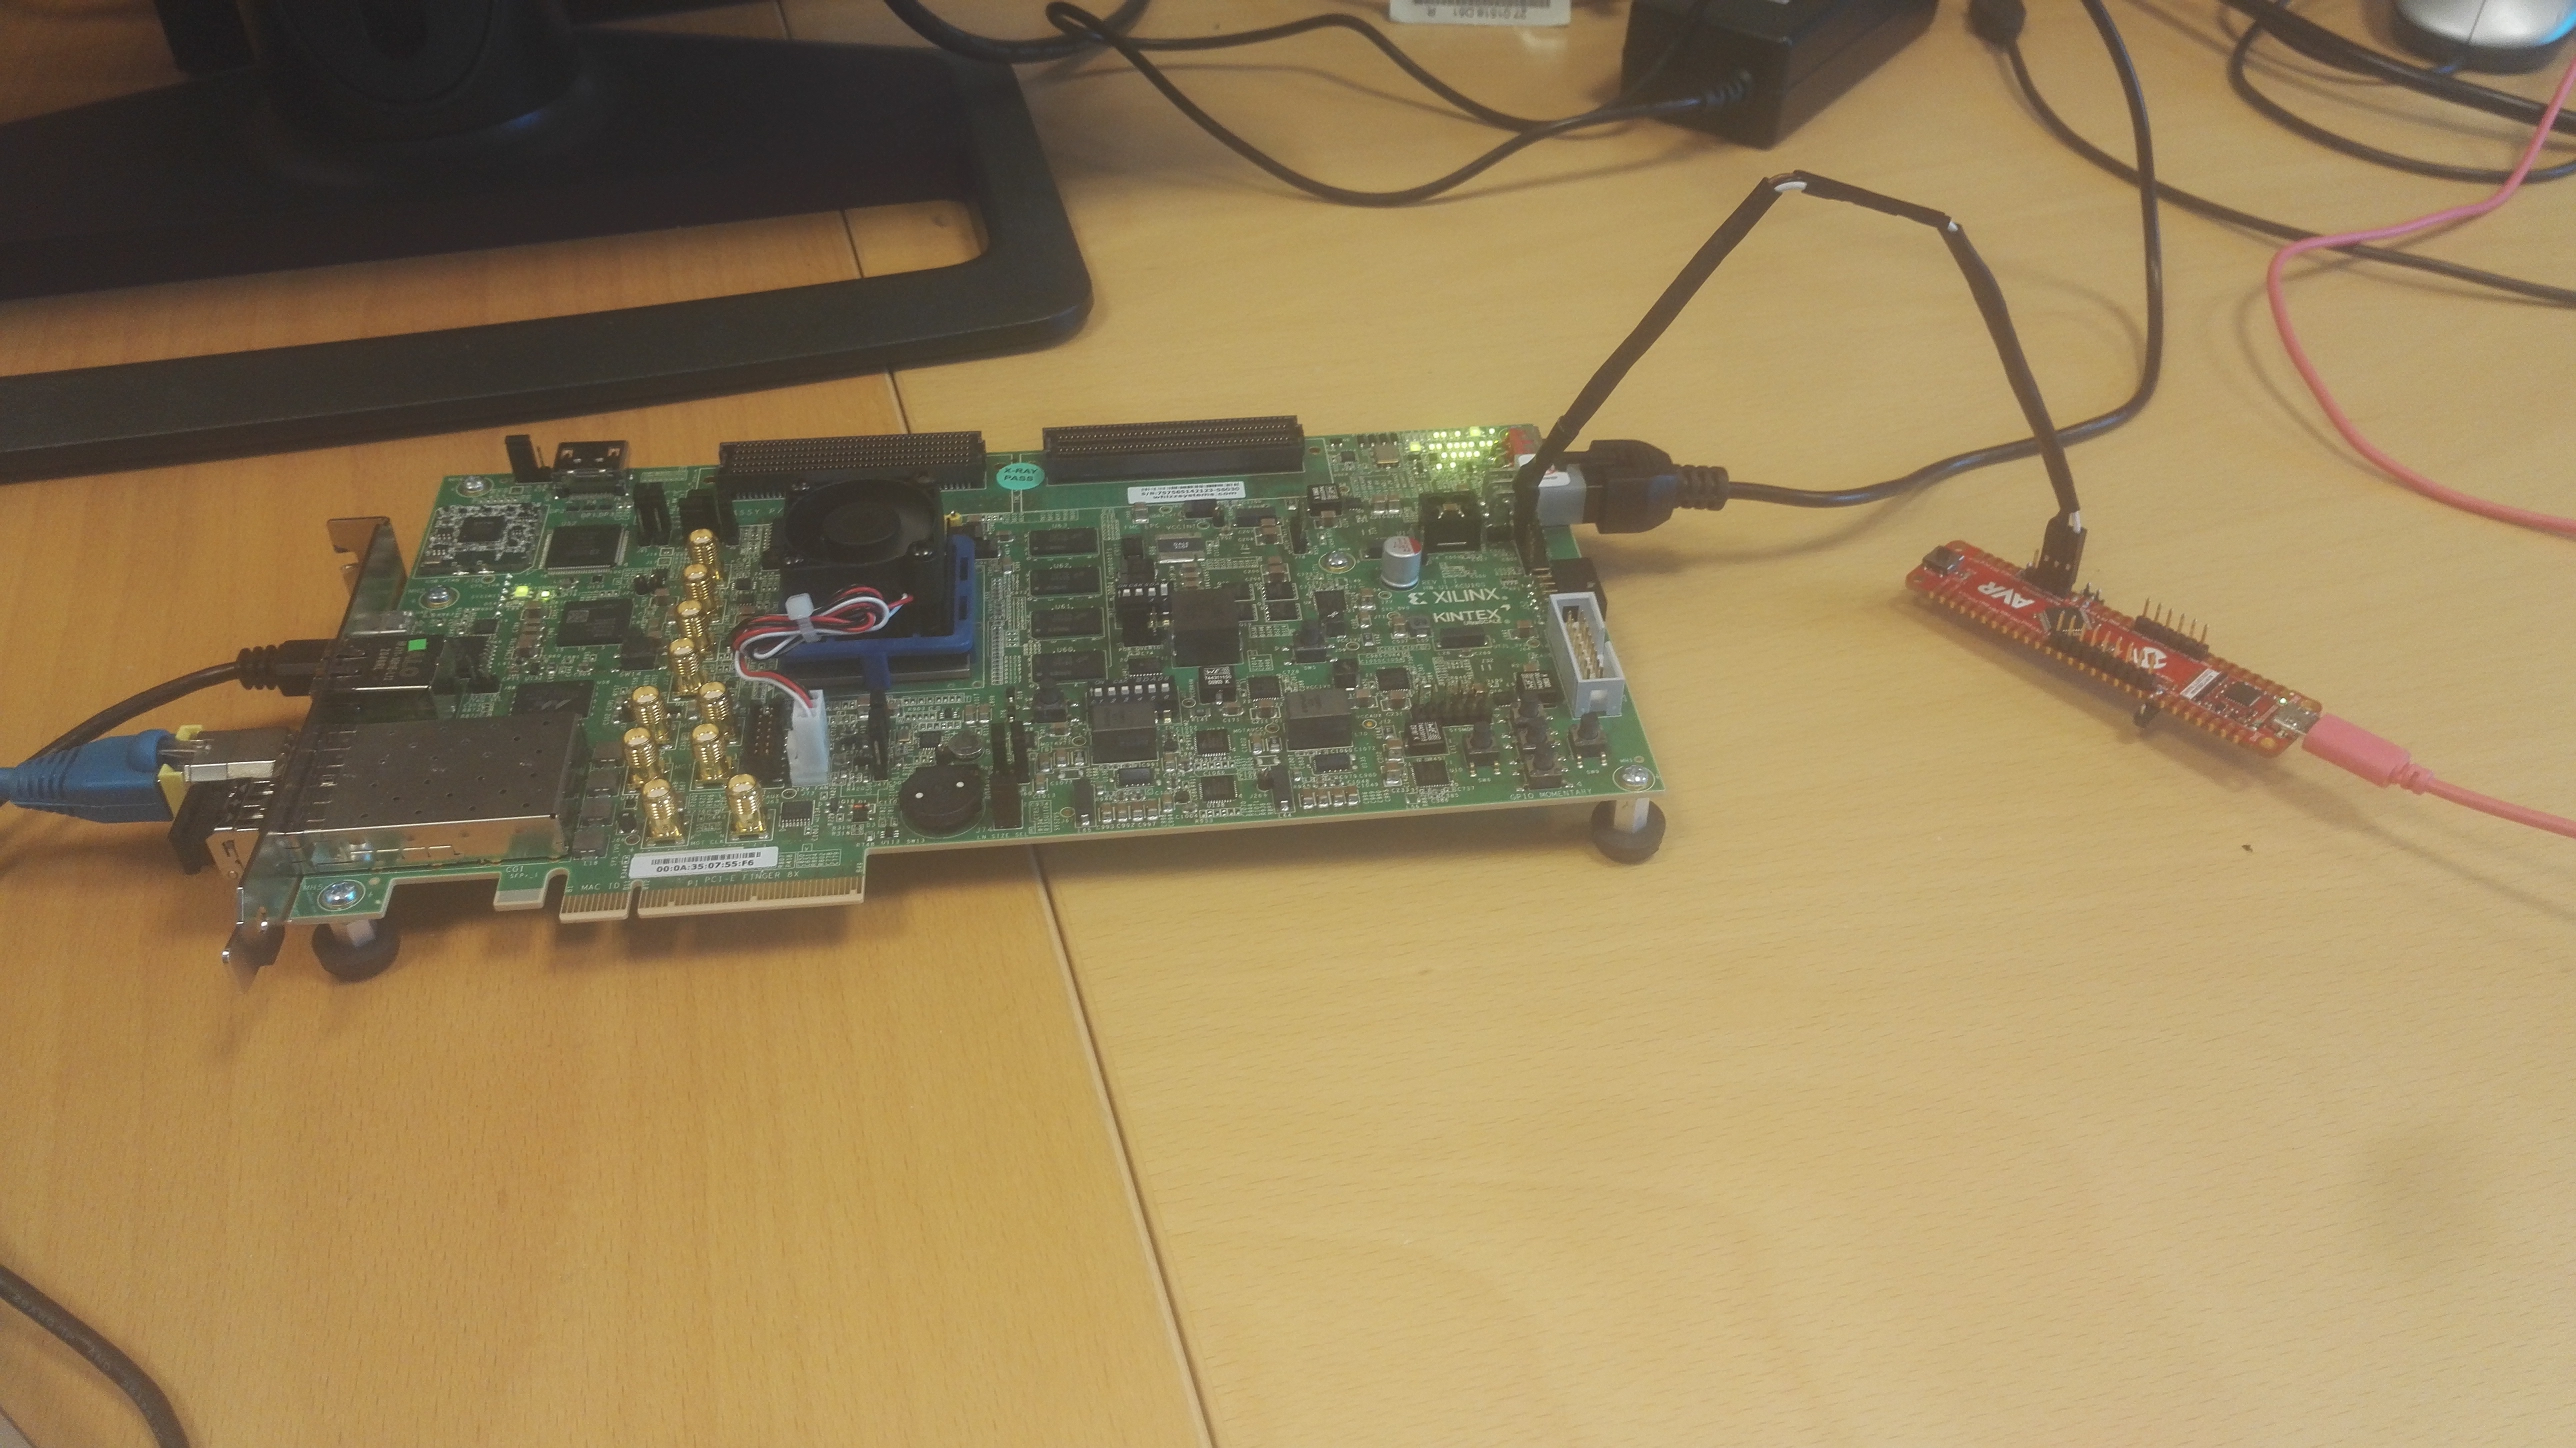
\includegraphics[width=14cm]{images/pcs_setup.jpg}
    \caption{PCS prototype setup.}
    \label{fig: pcs_setup}
\end{figure}
\FloatBarrier

The communication between the different parts of the prototype has been verified many times, but bit error rate tests that is discussed in \autoref{ssec: bit_error} shows that the reliability of the setup is inconsistent. This would suggest that this prototype should be improved or be made with more rigid components to ensure the test environment does not change over time. The fault lies between the \gls{fpga} and microcontroller so a solution could be to build a rigid connection between or put the microcontroller on an actual board to prevent it from moving.

Another problem with the test setup is the wire length between the evaluation board and microcontroller. The final product will use 3 metres of wire between them, but the test setup is only about 20 cm of wire. The length of the wire determines the resistance in it, and can affect signal transmission quality. For a new test setup in the future, longer wires should be used.



\subsection{Bit Error Rate}
\label{ssec: bit_error}
The bit error rate that occurs while sending data from control software to microcontroller must be verified and ensured is within an acceptable rate. Each data transferal goes through IPbus down to the \gls{fpga} and then \gls{fpga} relays the data to the microcontroller through standard \gls{usart} protocol.

We know that IPbus has a negligible error rate\cite{IPbus}, so any errors stemming from the \gls{fpga} will most likely come from the implementation of the \gls{fpga} design. The \gls{fpga} design itself is relatively simple by itself and as such, we will assume that all erroneous bits comes from the \gls{usart} communication between the \gls{fpga} and microcontroller.

When looking for errors in the data sent, we must be aware of where the data originates, if it is data from the \gls{fpga} then it will almost always be no errors. \autoref{fig: handshake_vals} shows how the data is processed between \gls{fpga} and microcontroller during a transaction, and from that we can see that almost all data in the RX register comes from the microcontroller. The only exception to this is during a write operation, where the \gls{fpga} will insert the data it sent to the RX register. The data bits during a write operation is therefore unimportant and does not tell us anything about the connection between \gls{fpga} and microcontroller. Testing for bit error rates using the write operation will therefore give us a bad coverage of the tested bits.

Testing for bit errors should be performed using the read operation, additionally, to ensure good test coverage, multiple bit patterns should be used to test edge cases like alternating bits, all 1's, all 0's or random bit pattern.

The test is done by performing a write to a microcontroller register that can be written and read from, we then perform 1000 read operations from said register. This gives one sample, and this test is done a variable amount more times to give us a mean error rate. Two versions of the test script is created, one where the number written is user defined, and the other uses random bit patterns for each run. Results of different bit patterns is given from \autoref{fig: all_0_bit_rate} to \ref{fig: rand_bit_rate}.

\begin{figure}[!ht]
    \centering
    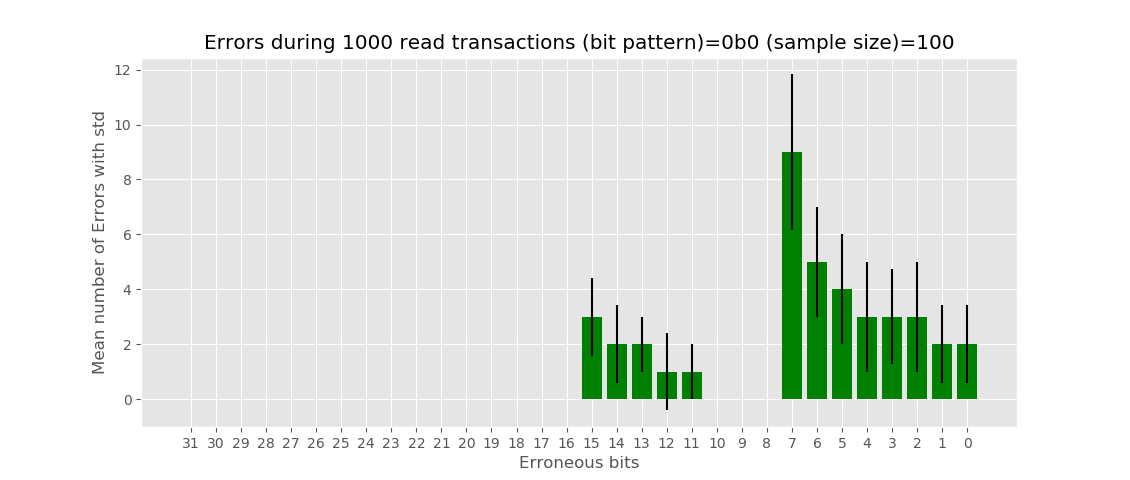
\includegraphics[width=18cm]{images/error_rate_all_0s.png}
    \caption{Histogram showing bit error rate with all 0's bit pattern.}
    \label{fig: all_0_bit_rate}
\end{figure}
\FloatBarrier

\begin{figure}[!ht]
    \centering
    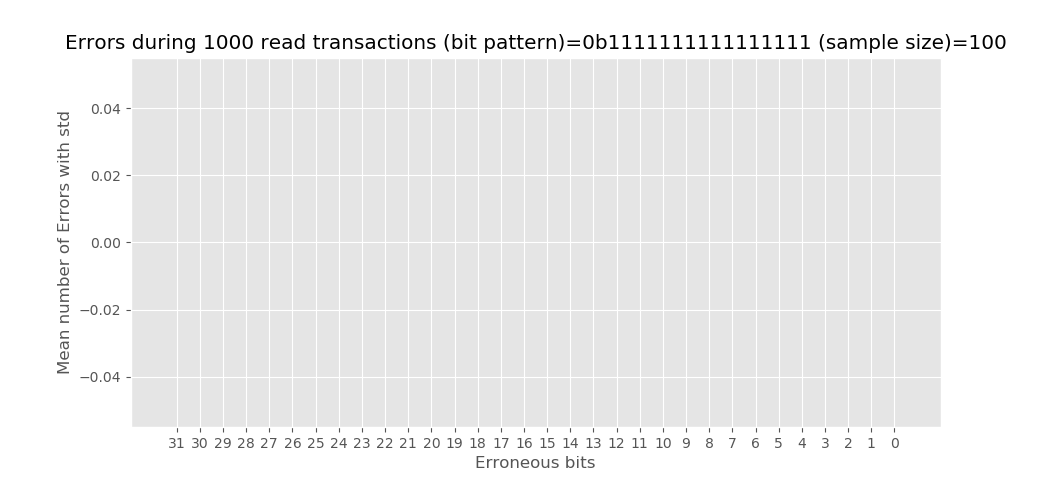
\includegraphics[width=18cm]{images/error_rate_all_1s.png}
    \caption{Histogram showing bit error rate with all 1's bit pattern.}
    \label{fig: all_1_bit_rate}
\end{figure}
\FloatBarrier

\begin{figure}[!ht]
    \centering
    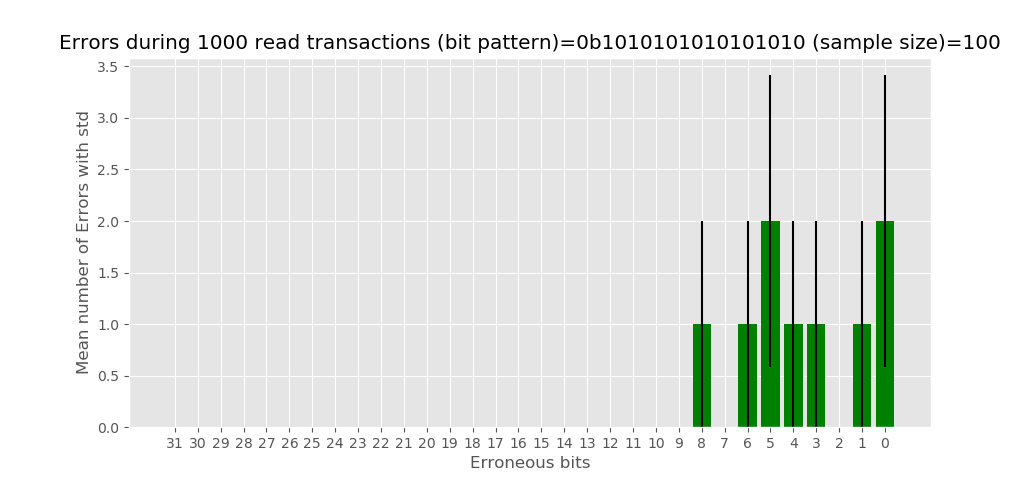
\includegraphics[width=18cm]{images/error_rate_alternating_1s.png}
    \caption{Histogram showing bit error rate with alternating 1's bit pattern.}
    \label{fig: alternating_1_bit_rate}
\end{figure}
\FloatBarrier

\begin{figure}[!ht]
    \centering
    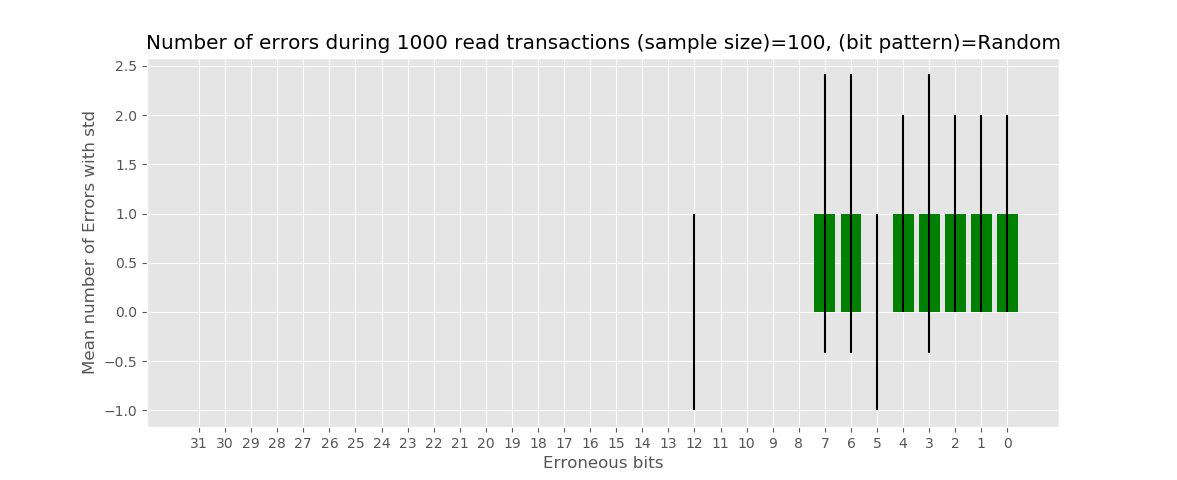
\includegraphics[width=18cm]{images/error_rate_random.png}
    \caption{Histogram showing bit error rate during a random bit read operation.}
    \label{fig: rand_bit_rate}
\end{figure}
\FloatBarrier

Important to note that the baud rate is set to 921600 for these tests. From the test results we can see that all but the "all 1's" test gave us errors. Alternating 1's and random bit pattern have a similar error pattern, they match well if we consider the standard deviation of the error measurements. All 0's gave a significant higher error rate than the other patterns, with worst bit error at 9 for bit 7. 9 bit errors for every 1000 reads results in an error rate of almost 1\%, which is an unacceptably high error rate. Even the alternating and random bit patterns have 1 error on several bits for every 1000 read, which is still unnaturally high.

The all 1's pattern is the outlier, having no errors during the entire test. That, combined with the all 0's pattern having abnormal amounts of errors, we must assume that the cause of the errors is misinterpreting 0's to be 1's. In other words, the sampling timing is not the inherent cause of the errors. Judging from the bits that have errors, only the data bits(15:0) have errors, but other than that, no obvious pattern gives us more insight into the errors.

Previous tests of the prototype did not suffer from any errors in the bit, and as such the most probable cause of the errors is due to inconsistent test environment. Due to time constraints, further tests and troubleshooting were not done, but the underlying issue most likely comes from uneven ground levels between \gls{fpga} and microcontroller, since the bit flip is always a zero turning into a one, never the other way.

\subsection{Baud rate error rate}

Another aspect of the \gls{pcs}-prototype that was tested was using different baud rates for the transmission between \gls{fpga} and microcontroller. If erroneous bits is caused by the sampling not hitting the falling edge of the clock, reducing the baud rate should improve the error rate, giving more time for sampling each bit. We observed in the previous section that there were an error rate of about 0.1\% for the data bits. This was tested with a baud rate of 921600. A test was performed to assess whether a lower baud rate improves the bit error rate. We can manually change the baud rate used in the transmission by writing to a register in the global module on the \gls{fpga}. The result of the test is given in \autoref{fig: baud_error}.

\begin{figure}[!ht]
    \centering
    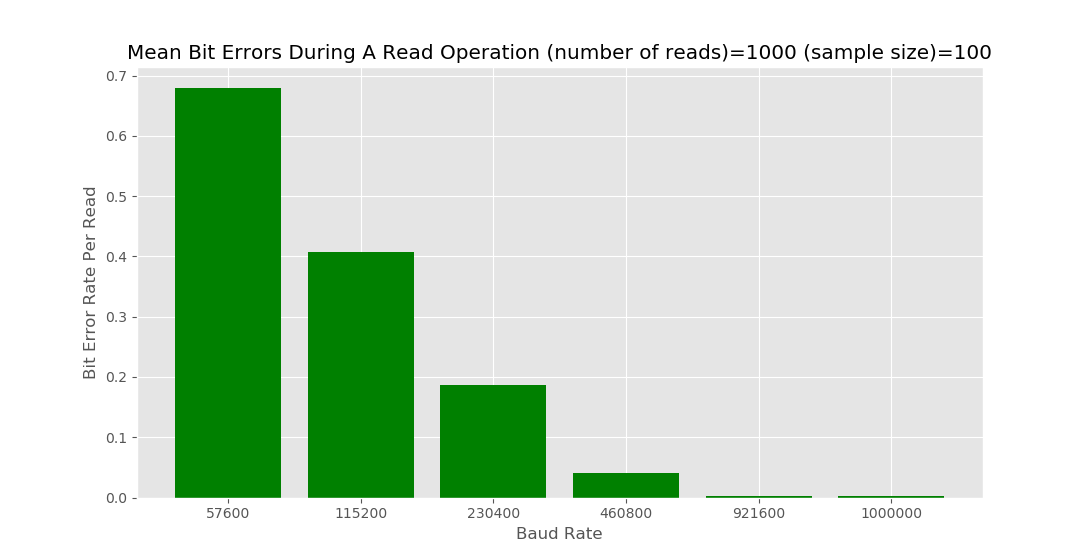
\includegraphics[width=18cm]{images/baud_error_rate.png}
    \caption{Histogram showing the amount of errors expected in one transaction for different baud rates.}
    \label{fig: baud_error}
\end{figure}
\FloatBarrier

From the figure, we can see that the lower baud rates in fact, increase the error rate, not lower it. The error rate increased from 0.1\% to a whopping 70\% on average for the lowest baud rate tested. This is an unexpected result which contradicts the behaviour of standard \gls{usart}s. This issue was present even before the uneven ground level issue that caused the errors in the previous section. The cause of this is not yet known, the cause may come from certain processes in the microcontroller taking too long for the system when it is using a lower baud rate. Another explanation for the errors can seen by observing the actual \gls{usart} communication with an oscilloscope. \autoref{fig: usart_com} shows the \gls{usart} communication between the microcontroller and \gls{fpga} while performing a read operation.

\begin{figure}[!ht]
    \centering
    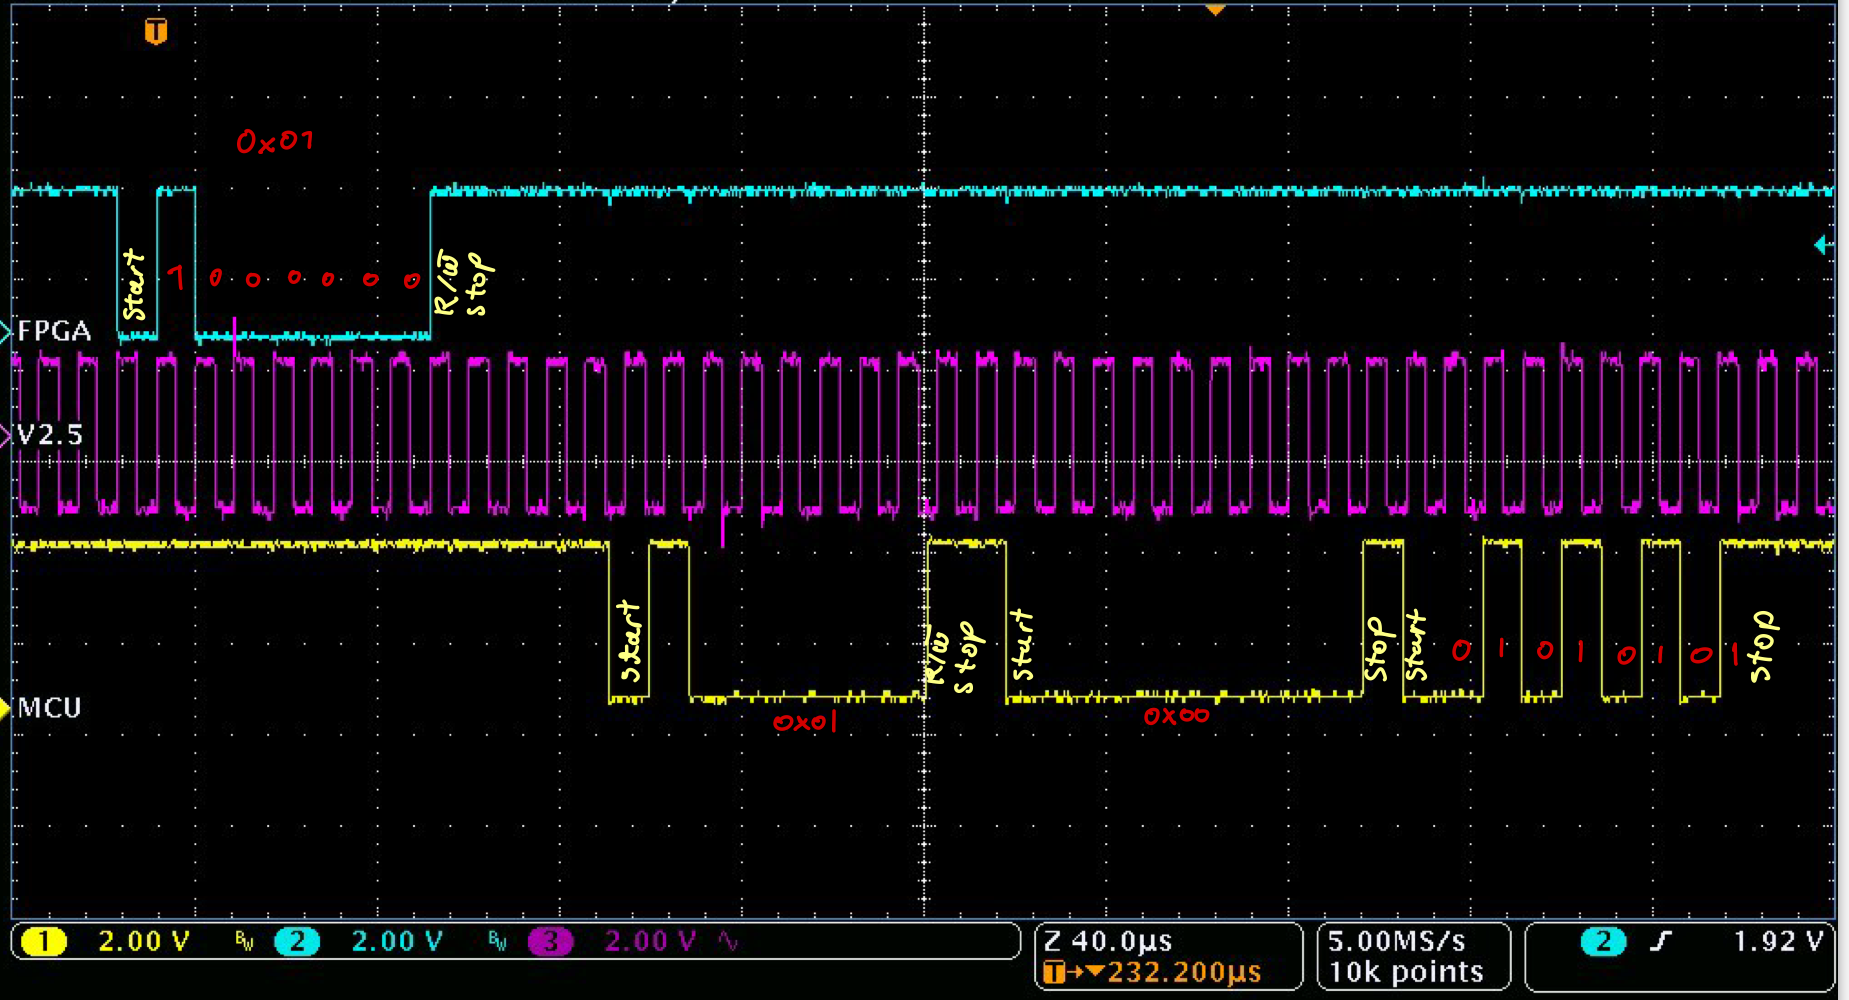
\includegraphics[width=18cm]{images/USARTTransaction.png}
    \caption{Oscilloscope image of the FPGA sending a read request to the microcontroller and receiving the data. Captured with a baud rate of 921600.}
    \label{fig: usart_com}
\end{figure}
\FloatBarrier

The figure shows the \gls{fpga} sending the read request, the microcontroller then performs a handshake by sending the read request back to the \gls{fpga}. After this it starts transmitting the data inside the two registers associated with address 0x01, which in this case is 0x00 and 0xAA. A possible explanation to the error rate can be seen then by observing the sampling of the data from the microcontroller. The microcontroller sends data on the rising edge of the clock, but there is a small random deviation on the microcontroller's timing for each bit read. This inconsistency could possibly cause issues for communication using lower baud rates. It is recommended to capture the \gls{usart} communication at lower baud rates to observe if this deviation causes issues. This is not been done due to time constraints.

The conclusion from this is that until the underlying issue is resolved, one should use as high baud rate as possible to avoid excessive errors. The microcontroller supports baud rates up to 1 000,000 and the standard baud rate closest to it is 921600. Higher baud rates also comes with the advantage of making the transmission speed faster, which is favorable for the \gls{pcs} design.

\subsection{Testbench}

To verify the functionality of the \gls{api}s and classes designed for the control software, testbenches have been made to test and verify the different functions. The focus is on testing the complex or specialized functions, tests for small, simple functions is deemed redundant and unnecessary and therefore not tested in the testbenches.

Due to the microcontroller software not being complete and not having access to the layers themselves, functions testing the entire \gls{pcs} chain has not been made, this means we do not have full test coverage on the tests. Additionally, tests for the \gls{pcs}-chain is not reliable due to the high bit error rate discussed in this chapter.

Testing the entire system can still be done by booting up the main hub \gls{gui} and observing that the control software behaves as expected. When all parts of the \gls{dtc} is available for testing, and the bit error rate is at an acceptable level, a full scale, automatic testbench should be developed, that allows for the entire system to be quickly tested and verified. This would serve as a standard for the system and allow for quick verification when modifying or expanding existing functions.

\subsection{Git and GitHub}

The use of the Git and GitHub tools is essential today to manage your code, maintain it and also as a version control system. Git is another method used to ensure that the code is easy to use and be maintained, now and in the future. The version control system is also essential for verifying the code, mistakes can be made, but a stable version of the software will always be available at the GitHub. GitHub also enables a better workflow with co-developers or mentors, allowing easy access to the source code and issues can be made. There is currently only one master branch of the repository in the Git system, this is due there only being one developer so branching is not yet needed.

The GitHub repository contains a README-file which contains all practical information about the repository and the goals of the project. This includes information about the configuration and monitoring process, as well as a user guide to start the databases and \gls{gui}. An example of the README-file is given in \autoref{fig: readme}


\begin{figure}[!ht]
    \centering
    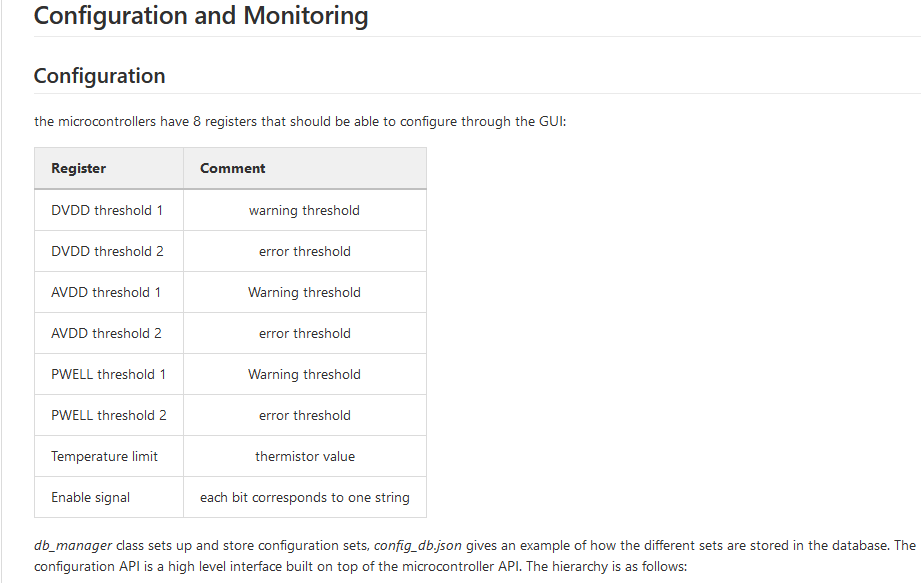
\includegraphics[width=18cm]{images/README_example.png}
    \caption{Example from the README-file showing the overview of the configuration process.}
    \label{fig: readme}
\end{figure}
\FloatBarrier

\subsection{Simulation}

The FPGA-design and the \gls{mb}-design is still in development during this thesis, and as such, we were unable to test and verify different components of the configuration and monitoring system. A solution to this problem is to create a simulation that mimics the behaviour of the system. The goal of the simulation is to create an adequate testing environment for the GUI and APIs developed and also allow for testing and familiarizing with IPbus itself. This involves the ability to read/write data from IPbus and process the data bit-wise. From the data it will determine if it is a read or write request and transmit the requested the data to the virtual address register. The code written for the simulation will also be similar to the actual implementation, allowing the code to be reused.

The simulation is written in python, using OOP template, meaning each module of the PCS has its own defined class with functions and encapsulated variables. Due to it being a direct connection between object class and its physical counterpart, expanding the simulation's functionality and adding new functions is intuitive and relatively easy to do.

\subsection{Overview}
As mentioned, the simulation is object-oriented, and is made of 4 classes and test functions for each of them. The classes are based on the final FPGA-design considered in \ref{section: fpga_design}. The FPGA itself is represented by the \textit{monitor sim manager} which instantiates a \textit{monitor module} object and a \textit{global module} object inside itself. The class representing the micro-controller is instantiated inside each monitor module class, mimicking how each module on the FPGA maintains its respective micro controller. Finally, \textit{monitor sim manager} is instantiated in the GUI class that is connected to the mongoDB API. This allows for testing the GUI and configuration of the micro-controllers in the simulation.  A class diagram of the simulation is shown in \ref{fig: class_diagram}.

\begin{figure}[!ht]
    \centering
    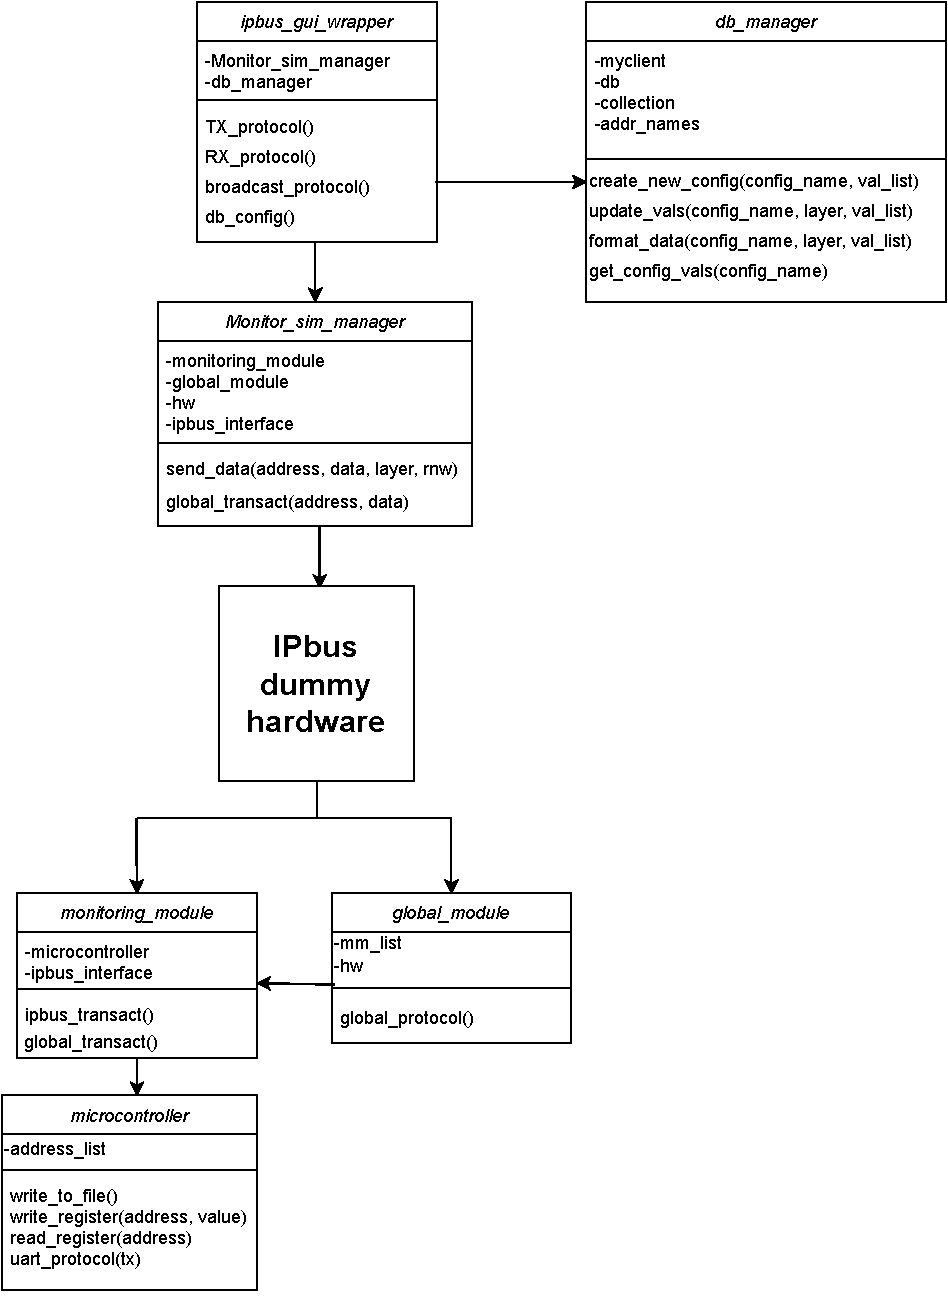
\includegraphics[width=14cm]{images/class chart.pdf}
    \caption{Class diagram of the simulation, including attributes and variables.}
    \label{fig: class_diagram}
\end{figure}
\FloatBarrier

\notinmain{snakke om i denne sectionen: features present and not present, limitations, uart communication is not simulated, fifos not simulated either, ingen FIFO. Bør eg endre simulasjonen til å lese data fra tekstfilene?}

\subsection{Features}

The simulation uses IPbus dummy hardware to communicate between the monitor sim manager class and the monitor module class. The dummy hardware is hosted on localhost of the computer and has the same functionality as of an IPbus module on a FPGA.  The number of layer modules and registers in the simulation is generic and can be set by the user upon instantiating the object, although the appropriate amount of modules must be manually added to the IPbus address map.

The FPGA and micro-controller class is able to perform read and write operations down to the virtual registers in the micro-controller class. The micro controller class decodes read/write bit, address and data from the TX value it is given, according to the data header discussed in \autoref{ssec: microcontroller}. A global module is also simulated, allowing for transmitting to every micro-controller by using the global transact function in the monitor sim manager. 

Using the simulation is as simple as instantiating the monitor sim manager object in the code and using the send data function to send TX data. The function will return the data from the specified RX register in IPbus. The micro-controller class will create a text file with its addresses and their contents, allowing the user to verify the data was correctly sent down to it.

\subsection{Limitations}

The simulation is built using python software and certain features is not able to be easily implemented. The USART communication protocol between the monitor module and micro-controller is omitted due to being relatively complicated to implement and for this purpose, not needed for testing GUI and API. 
The timing of data transfer is not considered in the simulations, meaning tasks such as data transfer between monitor module and micro-controller happens much faster than in the actual hardware. simulating timing is difficult to simulate using sequential code, since the actual hardware uses combinational logic that runs in parallel. We also have a prototype of the PCS chain which allows for more accurate speed tests than what a simulation could achieve. 





\end{document}